\documentclass[11pt]{article}
\pdftrailerid{}
\usepackage[T1]{fontenc}
\usepackage{lmodern}
\usepackage[margin=1.05in]{geometry}
\usepackage{amsmath,amssymb,amsthm,mathtools,microtype}
\usepackage{enumitem,xcolor,tikz}
\usetikzlibrary{arrows.meta,calc,positioning}
\usepackage[colorlinks=true,linkcolor=blue!45!black,citecolor=blue!45!black,urlcolor=blue!45!black]{hyperref}
\setlength{\emergencystretch}{2em}
\setlist{itemsep=3pt,topsep=5pt}
\newcommand{\C}{\mathbb C}
\newcommand{\Z}{\mathbb Z}
\newcommand{\N}{\mathbb N}
\newcommand{\Pp}{\mathbb P}
\newcommand{\Tot}{\operatorname{Tot}}
\newcommand{\Pic}{\operatorname{Pic}}
\newcommand{\mult}{\operatorname{mult}}
\newcommand{\ord}{\operatorname{ord}}
\newcommand{\W}{\mathcal W}
\newtheorem{theorem}{Theorem}[section]
\newtheorem{lemma}[theorem]{Lemma}
\newtheorem{proposition}[theorem]{Proposition}
\newtheorem{corollary}[theorem]{Corollary}
\theoremstyle{definition}
\newtheorem{definition}[theorem]{Definition}
\newtheorem{remark}[theorem]{Remark}
\numberwithin{equation}{section}
\title{Nagata's conjecture for plane curves}
\author{OpenAI}
\date{September 23, 2026}
\hypersetup{pdftitle={Nagata's conjecture for plane curves},pdfauthor={OpenAI}}
\begin{document}
\maketitle
\begin{abstract}
We prove that a nonzero effective plane curve of degree $d$ at $r\ge10$
very general complex points has total multiplicity strictly less than
$d\sqrt r$. The inequality holds simultaneously for all curves, including
reducible and nonreduced curves, and establishes Nagata's conjecture in
its strict, nonhomogeneous form.
\end{abstract}
\section{Introduction}\label{sec:introduction}

Prescribing multiple points of a plane curve is an interpolation problem:
how small can its degree be when the positions and the required orders of
vanishing are given? Nagata's conjecture predicts the answer at the
square-root scale for sufficiently many very general points. Nagata
introduced the problem in his work on Hilbert's fourteenth problem and
proved the square cases $r\ge16$~\cite{Nagata1959,Nagata1965}. We prove
the strict inequality for every $r\ge10$, allowing unequal multiplicities.

We first work over $\C$. Let
\[
 U_r=\{(p_1,\ldots,p_r)\in(\Pp^2_\C)^r:p_i\ne p_j\text{ for }i\ne j\}.
\]
A nonzero effective plane curve is the zero divisor of a nonzero
homogeneous form of degree $d\ge1$. Its multiplicity at a point is the
order of that form in the regular local ring. Components may repeat.
The phrase \emph{very general} in the following theorem means the
complement of one countable union of proper closed subsets, chosen
simultaneously for all degrees and multiplicity vectors.

The scale can already be seen when all prescribed multiplicities equal
$m$. A degree-$d$ form has $\binom{d+2}{2}$ coefficients, and order at
least $m$ at $r$ points imposes at most $r\binom{m+1}{2}$ linear
conditions. Their leading terms balance at $d=m\sqrt r$. A count of
conditions supplies curves asymptotically above this scale; proving their
absence below it requires control of the dependencies among the conditions, for every
$m$. The strict endpoint also matters: at nine points a nonzero cubic
always exists, so the asserted strict inequality cannot start at $r=9$.

\begin{theorem}\label{thm:main}
For every integer $r\ge10$, there is a countable union $E_r$ of proper
Zariski-closed subsets of $U_r$, with nonempty complement, such that the
following holds for every tuple $(p_1,\ldots,p_r)\notin E_r$.
If $C$ is a nonzero effective plane curve of degree $d\ge1$ and
$m_1,\ldots,m_r\in\Z_{\ge0}$ satisfy $\mult_{p_i}C\ge m_i$, then
\[
 d\sqrt r>\sum_{i=1}^r m_i.
\]
\end{theorem}

On the blowup of the plane at such a tuple, the theorem gives a real divisor
class of self-intersection zero that intersects every curve positively.
It also determines the multipoint Seshadri constant: the largest $t$ for
which the pullback of a line minus $t$ times the sum of the exceptional
curves has nonnegative intersection with every curve. Its value is
$1/\sqrt r$, which is irrational when $r$ is nonsquare.
Section~\ref{sec:consequences} proves these consequences
and extends the theorem to every uncountable algebraically closed field
of characteristic zero.

\subsection{Prior work and the interpolation approach}

The geometry of plane linear systems connects this problem with the cones
of effective and nef divisor classes on blowups. Ciliberto--Harbourne--
Miranda--Ro\'e~\cite{CHMR2012} develop these connections and compare
several forms and extensions of Nagata's conjecture.
For homogeneous multiplicities, Ro\'e~\cite{Roe2001} obtained the
uniform estimate $d>m(\sqrt{r-1}-\pi/8)$ for $r\ge10$ by
specializing to configurations with infinitely near points.
Harbourne~\cite{Harbourne2001} sharpened rational lower bounds and
proved further cases in restricted multiplicity ranges.
For ten very general points, degeneration methods give
$d/m\ge117/37$ for every nonempty homogeneous system: Eckl's Seshadri estimate and
Ciliberto--Dumitrescu--Miranda--Ro\'e's analysis of plane systems
give this bound in their respective formulations~\cite{Eckl2011,CDMR2011}.
Such bounds explain the importance of controlling arbitrarily large
multiplicities at each fixed nonsquare $r$.

Dumnicki--Harbourne--K\"uronya--Ro\'e--Szemberg~\cite{DHKRS2016}
study an analogue for very general monomial valuations, while
Nivoche~\cite{Nivoche2019} relates the conjecture to transcendental
interpolation in $\C^n$. These perspectives emphasize that the obstruction
is not merely the number of imposed conditions, but how vanishing
conditions interact with the geometry of the ambient surface.
More recently, Ciliberto--Miranda--Ro\'e~\cite[Theorem~1]{CMR2026}
constructed irrational square-zero nef rays on the blowups at every
$r\ge10$ very general points. Those constructions do not determine the
equal-weight multipoint Seshadri constant. Nagata's conjecture singles out
the class with equal exceptional coefficients, whose nefness gives that
constant's exact value.

The proof below uses two established approaches to this interaction.
Ciliberto--Miranda~\cite{CM1998} develop degenerations of plane linear
systems, and Evain~\cite{Evain2007} studies their infinitesimal limits
when fat points, meaning points equipped with specified orders of
vanishing, approach a divisor. Dumnicki~\cite{Dumnicki2007} encodes
interpolation by finite diagrams of monomial exponents and their
evaluation matrices. In particular, the proof of his Proposition~13 converts a
one-point derivative matrix into polynomial evaluation on the exponent
diagram. Our final rank problem has the same evaluation interpretation,
with a different set of allowed polynomial degrees supplied by a
collinear collision.

The elliptic stage uses the classical multiplicative theta product and
its residue-class Laurent bases; the conventions used here are recorded
in Rosengren~\cite[arXiv version, Section~1.2 and Exercise~1.6.5]{Rosengren2020}.
We prove the needed product identities, basis formulas and convergence
estimates in the normalization required by the argument.

\subsection{Proof strategy}

Closed incidence loci turn a failure at very general points into a
system of curves existing at every configuration. A product over cyclic
permutations makes the multiplicities equal; write $d$ and $m$ for the
resulting degree and common multiplicity. Moving the points toward a
smooth curve gives a nonzero polynomial on its normal line bundle,
with order at least $m$ at arbitrary normal displacements. For square
$r$, its two highest coefficients already exclude $d/m\le\sqrt r$,
including equality (Section~\ref{sec:reductions}).

For nonsquare $r$, we use a cubic and set nine normal displacements to
zero. Dividing out the forced coefficient zeros and changing the fiber
coordinate give a finite-dimensional space of polynomial sections whose
first $m+1$ coefficient bundles have equal degree
(Section~\ref{sec:elliptic}). On each fixed elliptic curve, the remaining
$q=r-9$ points collide along a horizontal coordinate line. After $b<m$
fiber derivatives, a section must then have base order at least $q(m-b)$;
thus a particular finite jet map has a nonzero kernel. A separate
degeneration gives explicit normalized theta bases whose expressions
in logarithmic base and fiber coordinates $(x,y)$ tend to $e^{Kx+jy}$.
Here $j$ is the fiber degree and $K$ a Laurent exponent. Their mixed
derivatives give the limiting matrix
\[
 \bigl(K^\ell j^b\bigr),\qquad
 0\le b<m,\quad 0\le\ell<q(m-b),
\]
with columns indexed by exponent pairs $(j,K)$
(Section~\ref{sec:limits}). Only these numerical matrices are compared
across curves; the argument does not choose a simultaneous family of
kernel vectors.

To exclude the kernel, a total count of exponent pairs is not enough.
We group them into horizontal rows of fixed $K$, with $j$ varying.
Interpolation one row at a time gives full column rank if no row has
more than $m$ points and at most $q(m-t+1)$ rows have at least $t$ points.
The exponent pairs lie in a polygon whose slice-width profile supplies
exactly these bounds. Since $d/m$ is rational and $r$ is nonsquare,
the strict gap $d/m<\sqrt r$ permits a contraction of that polygon;
taking a common power of the original curve absorbs the integer endpoint
error in the row count. Full rank persists for small positive degeneration
parameter, contradicting the kernel on each fixed curve
(Section~\ref{sec:interpolation}).

\section{From plane curves to normal polynomials}
\label{sec:reductions}

We reduce a violation at very general points to an equal-multiplicity
system existing at every configuration.  Moving its points toward a
smooth plane curve then gives a polynomial on the normal bundle.
This polynomial will exclude the square cases and supply the input
for the cubic construction in Section~\ref{sec:elliptic}.

The order of a section is the order of its scalar expression in a local
frame.  A frame change multiplies this expression by a unit, preserving
the order.  In local coordinates, order at least $m$ means that every
Taylor coefficient of total degree less than $m$ vanishes.  Thus
algebraic and holomorphic orders agree, and holomorphic coordinate
changes preserve them.

\subsection{A universal equal-multiplicity system}

For positive integers $d,m$, write $\mathsf U_r(d,m)$ for the property
\begin{equation}
\label{eq:universal}
\begin{gathered}
\text{For every }(p_1,\ldots,p_r)\in U_r\text{ there is a nonzero form}\\
S\in H^0(\Pp^2,\mathcal O_{\Pp^2}(d))
\quad\text{such that}\quad
\mult_{p_i}(S)\ge m\quad(1\le i\le r).
\end{gathered}
\end{equation}
Here and below the multiplicity of a form is the multiplicity of its
zero divisor.

\begin{lemma}[Reduction to universal systems]
\label{lem:universal}
For each $r\ge10$ there is a countable union $E_r$ of proper
Zariski-closed subsets of $U_r$, all defined over $\mathbb Q$, with
$U_r\setminus E_r\ne\varnothing$, having the following property.
If a tuple outside $E_r$ supports a
degree-$d_0$ form, $d_0\ge1$, with multiplicities at least
$m_1,\ldots,m_r\in\Z_{\ge0}$ and
\[
 d_0\sqrt r\le\sum_{i=1}^r m_i,
\]
then $\mathsf U_r(d,m)$ holds for some positive integers $d,m$ with
$d/m\le\sqrt r$.  If $\mathsf U_r(d,m)$ holds, then
$\mathsf U_r(Nd,Nm)$ holds for every positive integer $N$.
Consequently, to prove Theorem~\ref{thm:main} for a fixed $r$, it suffices
to rule out every $\mathsf U_r(d,m)$ with $d/m\le\sqrt r$.
\end{lemma}

\begin{proof}
For a positive integer $e$ and
$\mathbf n=(n_1,\ldots,n_r)\in\Z_{\ge0}^r$, let
$A_{e,\mathbf n}\subseteq U_r$ consist of the tuples admitting a nonzero
degree-$e$ form with multiplicity at least $n_i$ at the $i$th point.
In standard affine charts, the required Taylor coefficients give a
matrix with $\binom{e+2}{2}$ columns, one for each form coefficient.
Its entries are polynomials with integer coefficients in the point
coordinates.  A nonzero form exists exactly when the matrix has less
than full column rank.  Thus $A_{e,\mathbf n}$ is cut out by its
full-column-size minors; if there are fewer rows than columns, the
condition is automatic.  Invariance of order makes these rank
conditions agree on overlaps.  Consequently $A_{e,\mathbf n}$ is
Zariski closed and defined over $\mathbb Q$.

Let $E_r$ be the union of all proper $A_{e,\mathbf n}$.  This is a
countable union.  On the dense chart where all points are affine,
each proper $A_{e,\mathbf n}$ has a defining minor that is a nonzero
polynomial over $\mathbb Q$.  Choose
$2r$ complex numbers algebraically independent over $\mathbb Q$ as
affine coordinates of the marked points.  Such numbers can be chosen
successively, since the algebraic closure of a countable field is
countable.  None of these minors vanishes at the resulting tuple, which
also avoids the diagonals.  Hence it lies in $U_r\setminus E_r$.

Now suppose that a violation as in the statement occurs outside $E_r$.
Then $A_{d_0,\mathbf m}=U_r$.  We use the cyclic-product reduction of
Nagata~\cite{Nagata1965}.
Permuting the ordered points gives the
same assertion for each cyclic shift of $\mathbf m$.  At any fixed
tuple, choose a nonzero form for each of the $r$ cyclic shifts and
take their product.  This product is nonzero, and orders add because
the product of the initial Taylor terms is nonzero.  Each original
multiplicity occurs once at each point.  Hence the product has degree
and common lower multiplicity
\[
 d=rd_0,
 \qquad
 m=\sum_{i=1}^r m_i.
\]
The assumed violation makes $m>0$, and
\[
 \frac d m
 =\frac{r d_0}{\sum_i m_i}
 \le\sqrt r.
\]
The construction applies at every tuple, proving $\mathsf U_r(d,m)$;
taking $N$th powers proves the common-multiple assertion.  Thus
excluding these universal systems excludes every violation outside
the same $E_r$, for all degrees and multiplicity vectors.
\end{proof}

\subsection{Specialization to a normal bundle}

Let $B\subseteq\Pp^2$ be a smooth irreducible plane curve of degree
$k\ge1$, and fix a nonzero homogeneous equation $G_B$ for it.  Put
\[
 L=\mathcal O_B(1),\qquad M=L^k.
\]
The equation identifies the normal bundle of $B$ in $\Pp^2$ with $M$,
as in the formula for an effective Cartier divisor
\cite[Tag~0B3P]{Stacks}.  In a local frame $e$ for
$\mathcal O_{\Pp^2}(1)$, the local equation
$t=G_B/e^k$ identifies a normal vector with its derivative under $t$.
For $w\in M_a$, the expression $f_j(a)w^j$ is an element of $L_a^d$
when $f_j$ is a section of $L^{d-kj}$.  Thus the polynomial in the next
proposition is intrinsically a section of the pullback of $L^d$ to
$\Tot(M)$.

\begin{proposition}[A necessary normal polynomial]
\label{prop:normal-polynomial}
Suppose that $\mathsf U_r(d,m)$ holds.  For every choice of distinct
points $a_1,\ldots,a_r\in B$ and arbitrary vectors $c_i\in M_{a_i}$,
there is a nonzero polynomial
\begin{equation}
\label{eq:normal-polynomial}
 F(w)=\sum_{j=0}^{\lfloor d/k\rfloor}f_jw^j,
 \qquad f_j\in H^0(B,L^{d-kj}),
\end{equation}
having multiplicity at least $m$ at each $(a_i,c_i)\in\Tot(M)$.
Its coefficients may be taken to be algebraic sections.
\end{proposition}

\begin{proof}
We move the marked points in the plane, rescale the normal coordinate,
and retain the first nonzero term of a family of plane forms.

Choose a plane affine chart and its standard frame near each $a_i$.
The differential of the local equation $t_i$ is nonzero by smoothness,
so choose an affine tangent vector $V_i$ with $dt_i(V_i)=c_i$ in
that frame.  The affine-linear motions
\[
 p_i(s)=a_i+sV_i
\]
are rational in $s$, stay distinct for sufficiently small $s$, and satisfy
\[
 \lim_{s\to0}\frac{t_i(p_i(s))}{s}=c_i
\]
in the chosen frames.  The vectors $c_i$ are arbitrary complex
normal vectors; no compatibility among them is required.

Multiplicity at least $m$ at all $p_i(s)$ gives a homogeneous linear
system over $\C(s)$ in the degree-$d$ form coefficients.  It has a
nonzero solution: otherwise some full-column-size minor would be a
nonzero rational function, giving full column rank at general complex
values of $s$ and contradicting $\mathsf U_r(d,m)$.

Clear denominators in a nonzero rational solution, and divide its
polynomial coefficients by their maximal common power of $s$.  This
gives a finite polynomial family of homogeneous degree-$d$ forms
\[
 S(s)=\sum_{\alpha\ge0}s^\alpha S_\alpha,
 \qquad S_0\ne0,
\]
satisfying the required multiplicities for general $s$.  For each
nonzero $S_\alpha$, factor out its largest power of $G_B$:
\[
 S_\alpha=G_B^{j_\alpha}R_\alpha,
 \qquad
 0\le j_\alpha\le\lfloor d/k\rfloor.
\]
Then $R_\alpha$ has degree $d-kj_\alpha$ and $R_\alpha|_B\ne0$,
since the homogeneous ideal of $B$ is generated by $G_B$.
Set
\[
 u=\min_{S_\alpha\ne0}(\alpha+j_\alpha),
 \qquad
 F(w)=\sum_{\alpha+j_\alpha=u}
       (R_\alpha|_B)w^{j_\alpha}.
\]
The sum is nonempty, and its terms have distinct exponents $j_\alpha$
because $\alpha+j_\alpha=u$.  Thus $F$ is nonzero, with algebraic
coefficients of the types in \eqref{eq:normal-polynomial}.

It remains to identify this polynomial as the normal limit and pass
the multiplicities to it.  Near a marked point choose a frame $e$ for
$\mathcal O_{\Pp^2}(1)$, put $t=G_B/e^k$, and extend a local coordinate
on $B$ to a holomorphic coordinate $\zeta$ off $B$ so that $(\zeta,t)$
are surface coordinates.  Write $r_\alpha(\zeta,t)$ for the scalar
expression of $R_\alpha$ in the frame $e^{d-kj_\alpha}$.  Substituting
$t=sw$ in the local expression of $S(s)$ and dividing by $s^u$ gives
\[
 \Phi(s,\zeta,w)
 =\sum_{S_\alpha\ne0}
 s^{\alpha+j_\alpha-u}w^{j_\alpha}
 r_\alpha(\zeta,sw).
\]
Every exponent of $s$ is nonnegative, so $\Phi$ extends
holomorphically to $s=0$ with value $F$.  Terms with
$\alpha+j_\alpha>u$ vanish there; in the remaining terms only
$r_\alpha(\zeta,0)$ contributes.

The limit respects the normal-bundle and value-bundle frames.  Indeed,
if $e'=a(\zeta,t)e$, then $t'=a(\zeta,t)^{-k}t$ and the scalar
expression of the section is multiplied by $a(\zeta,t)^{-d}$.
After $t=sw$, the transitions at $s=0$ are
\[
 w'=a(\zeta,0)^{-k}w,
 \qquad
 F'=a(\zeta,0)^{-d}F.
\]
These are the transitions of $M$ and the pullback of $L^d$.
Changing the extension of $\zeta$ off $B$ reduces at $s=0$ to its
coordinate change on $B$, since the other terms contain $t=sw$.
Thus the local rescaling realizes the intrinsic polynomial $F$ above.

Finally fix an index $i$ and use such coordinates near $a_i$.  The
functions
\[
 \zeta_i(s)=\zeta(p_i(s)),
 \qquad
 w_i(s)=\frac{t(p_i(s))}{s}
\]
extend holomorphically to $s=0$, with values representing $a_i$ and
$c_i$.  Translate the divided family to the lifted moving point:
\[
 \Psi_i(s,\xi,\omega)
   =\Phi\bigl(s,\zeta_i(s)+\xi,w_i(s)+\omega\bigr).
\]
For each general nonzero $s$, the substitution $t=sw$ is a local
biholomorphism of the surface, and multiplication by $s^{-u}$ is
multiplication by a nonzero scalar.  The multiplicity assumption on
$S(s)$ therefore implies
\[
 \partial_\xi^a\partial_\omega^b
 \Psi_i(s,0,0)=0
 \qquad(a,b\ge0,\ a+b<m).
\]
Each expression on the left is holomorphic at $s=0$ and vanishes
for general nonzero $s$, hence also at zero.  These are exactly the
order-$m$ conditions for $F$ at $(a_i,c_i)$.
\end{proof}

\subsection{The square case}

We use two basic facts about smooth projective curves.  A nonzero
section of a line bundle has an effective zero divisor whose degree
is the degree of the bundle.  In particular, a degree-zero line
bundle has a nonzero section only if it is trivial.  Also, for a
smooth complex projective curve of positive genus, $\Pic^0(B)$ is
a complex torus; its subgroup of elements of any fixed finite order
is finite, so its torsion subgroup is countable~\cite[Tag~0C1Z]{Stacks}.

\begin{proposition}[Strict inequality for square $r$]
\label{prop:squares}
Let $r=k^2$ with $k\ge4$.  There are no positive integers $d,m$ such
that $d\le km$ and $\mathsf U_r(d,m)$ holds.
\end{proposition}

\begin{proof}
Suppose that $d\le km$ and $\mathsf U_r(d,m)$ holds.  We choose
the marked points to exclude normal polynomials of fiber degree below
$m$, and the displacements to exclude fiber degree $m$.
Take a smooth degree-$k$ plane curve $B$, for example a Fermat curve,
and retain $L=\mathcal O_B(1)$ and $M=L^k$.  Its genus is
$(k-1)(k-2)/2>0$, and $\deg M=k^2=r$.  Choose distinct points
$a_1,\ldots,a_r$ so that, with $P=\sum_i a_i$, the degree-zero bundle
\[
 A=M(-P)
\]
is nontorsion.  Such a choice exists: fix $r-1$ distinct points and
vary the last one.  The map $a\mapsto\mathcal O_B(a)$ is injective
on a positive-genus curve, since a linear equivalence between two
distinct single points would give a nonconstant meromorphic function
with one simple pole, hence a degree-one map to $\Pp^1$, making the
curve rational.  Thus varying the last point gives uncountably many
distinct bundles $A$, while the torsion bundles are countable; the
finitely many prohibited coincidences may also be avoided.

The restriction sequence
\[
 0\longrightarrow\mathcal O_{\Pp^2}
 \xrightarrow{\,G_B\,}\mathcal O_{\Pp^2}(k)
 \longrightarrow\mathcal O_B(k)\longrightarrow0
\]
and $H^1(\Pp^2,\mathcal O_{\Pp^2})=0$~\cite[Tag~01XT]{Stacks} give
\[
 h^0(B,M)=\binom{k+2}{2}-1
         =\frac{k^2+3k}{2}<k^2=r.
\]
Hence one can choose
$c=(c_i)_i\in\bigoplus_i M_{a_i}$ outside the image of the evaluation
map
\[
 H^0(B,M)\longrightarrow\bigoplus_{i=1}^r M_{a_i}.
\]

Apply Proposition~\ref{prop:normal-polynomial} with these choices.  Let $j$
be the largest exponent with $f_j\ne0$.  Then
$j\le\lfloor d/k\rfloor\le m$.  If $j<m$, take $j$ derivatives with
respect to a local fiber coordinate.  Since $j$ is the largest
exponent, the result is $j!f_j$, independent of the fiber coordinate.
Differentiation lowers order by at most $j$, so $f_j$ has base
vanishing order at least $m-j$ at each $a_i$.  Its bundle has degree
\[
 \deg L^{d-kj}=k(d-kj)\le k^2(m-j)=r(m-j).
\]
Strict inequality is incompatible with these required zeros.  Equality
forces $d=km$, and removing the zeros then gives a nonzero section of
\[
 L^{k(m-j)}\bigl(-(m-j)P\bigr)=A^{m-j}.
\]
This is a nontrivial degree-zero bundle, because $A$ is nontorsion and
$m-j>0$, so it too has no nonzero section.  Thus $j<m$ is impossible.

It follows that $j=m$ and $d=km$.  In this case $f_m$ is a nonzero
constant.  At each marked fiber the restriction of $F$ is a degree-$m$
polynomial, with leading coefficient $f_m$, having a zero of order at
least $m$ at $c_i$.  In any compatible frame it therefore equals
\[
 F|_{M_{a_i}}(w)=f_m(w-c_i)^m.
\]
Comparing the coefficient of $w^{m-1}$ gives
\[
 (f_{m-1}(a_i))_i=-m f_m(c_i)_i.
\]
But $f_{m-1}\in H^0(B,M)$, and multiplication by the nonzero scalar
$-m f_m$ preserves the image of the evaluation map.  This contradicts
the choice of $c$ and finishes the proof.
\end{proof}

Together with Lemma~\ref{lem:universal}, the proposition proves
Theorem~\ref{thm:main} for square $r$, including the strict inequality
and unequal multiplicities.

\subsection{Nine zero displacements on a cubic}

For the remaining argument we will apply
Proposition~\ref{prop:normal-polynomial} with $k=3$ and with zero
normal displacements at nine distinct points of a smooth plane cubic.
Write $P=a_1+\cdots+a_9$.  Extend the coefficient list by $f_j=0$
for $j>\lfloor d/3\rfloor$.  At each $(a_i,0)$, expansion in the
fiber variable shows that multiplicity at least $m$ implies
\begin{equation}
\label{eq:nine-zeros}
 f_j\in H^0\bigl(B,L^{d-3j}(-(m-j)P)\bigr)
 \qquad(0\le j<m).
\end{equation}
Indeed, in a local base coordinate $\zeta$ centered at $a_i$, the
coefficient of $\zeta^a w^j$ must vanish whenever $a+j<m$.
Thus $f_j$ has base order at least $m-j$ at every point of $P$.
The coefficient bundles in \eqref{eq:nine-zeros} all have degree
$3(d-3m)$, independent of $j$.  These conditions hold regardless of
the additional points and normal displacements chosen in the proposition.

\begin{lemma}[Excluding degree at most $3m$]
\label{lem:cubic-low-degree}
If $r\ge10$ and $\mathsf U_r(d,m)$ holds for positive integers $d,m$,
then $d>3m$.
\end{lemma}

\begin{proof}
Suppose first that $d<3m$.  Choose a smooth plane cubic and nine
distinct points with zero normal displacements, as above, completing
them to $r$ distinct base points with arbitrary further displacements.
Every exponent occurring in \eqref{eq:normal-polynomial} is less than
$m$.  For each such exponent, \eqref{eq:nine-zeros} prescribes at
least $9(m-j)$ zeros, whereas
\[
 \deg L^{d-3j}=3(d-3j)<9(m-j).
\]
Thus every coefficient is zero, contradicting the nonzero polynomial
provided by Proposition~\ref{prop:normal-polynomial}.

Now suppose that $d=3m$.  A smooth plane cubic has genus one.  Choose
the nine points so that $A=L^3(-P)$ is nontorsion, by the same
argument used in the square case.  Complete them to $r$ distinct
base points, choosing a nonzero vector $c_{10}\in M_{a_{10}}$;
this is possible because $r\ge10$.  Apply
Proposition~\ref{prop:normal-polynomial} with these choices and zero
displacements at the first nine points.
For every $j<m$, the bundle in
\eqref{eq:nine-zeros} is $A^{m-j}$, a nontrivial degree-zero bundle.
Hence these coefficients vanish, and the nonzero normal polynomial
must be $F(w)=f_mw^m$ for a nonzero constant $f_m$.  This is nonzero at
$(a_{10},c_{10})$, so it cannot have multiplicity at least $m\ge1$
there.  This is again a contradiction.
\end{proof}

\section{Polynomial sections on an elliptic curve}
\label{sec:elliptic}

Nine zero normal displacements impose zeros on the coefficients of a
normal polynomial. Dividing out these zeros puts its first $m+1$
coefficients in bundles of the same positive degree. We first make this
change intrinsically on any smooth cubic. We then choose cubics and
marked points for which theta functions give explicit bases of the
resulting spaces, ready for the collision and limit in
Section~\ref{sec:limits}.

In this section and Section~\ref{sec:limits}, $H^0$ denotes holomorphic
sections. The algebraic sections supplied by
Proposition~\ref{prop:normal-polynomial} belong to these spaces, so
excluding holomorphic solutions will also exclude the necessary normal
polynomials.

\subsection{Removing the nine prescribed coefficient zeros}

For this construction, let $d,m$ be any positive integers with $d>3m$.
Let $B$ be a smooth plane cubic, let $L=\mathcal O_B(1)$ and
$M=L^3$, and choose nine distinct points with divisor
$P=a_1+\cdots+a_9$. Write $\sigma_P$ for the canonical section of
$\mathcal O_B(P)$ with zero divisor $P$, and put
\[
 A=M\otimes\mathcal O_B(-P),\qquad
 T=L^{d-3m},\qquad u_0=\lfloor d/3\rfloor.
\]
Thus $\deg A=0$ and $\deg T=3(d-3m)>0$. Multiplication by
$\sigma_P$ defines a bundle map $A\to M$, written
\[
 w=\sigma_P v,
\]
which is invertible over $B\setminus P$. Define coefficient spaces
inside $H^0(B,T\otimes A^{m-j})$ by
\begin{equation}
 V_j=
 \begin{cases}
 H^0(B,T\otimes A^{m-j}),&0\leq j\leq m,\\[1mm]
 \sigma_P^{j-m}H^0(B,L^{d-3j}),&m<j\leq u_0.
 \end{cases}
\label{eq:coefficient-spaces}
\end{equation}
Negative powers denote dual powers. The target in the second line is
correct because
\[
 L^{d-3j}\otimes\mathcal O_B((j-m)P)=T\otimes A^{m-j}.
\]
Multiplication by $\sigma_P^{j-m}$ is injective, as can be checked on
$B\setminus P$. Let $\W$ be the space of polynomial sections on
$\Tot(A)$
\[
 \widetilde F(v)=\sum_{j=0}^{u_0}g_jv^j,\qquad g_j\in V_j,
\]
valued in the pullback of $T\otimes A^m=L^d(-mP)$.
It is a finite-dimensional space: its coefficient blocks are spaces of
sections on the compact curve $B$, and distinct powers of the fiber
coordinate make their sum direct.

The nine zero displacements are now built into $\W$. The remaining
points impose ordinary multiplicities at scalar fiber coordinate $1$,
as follows.

\begin{proposition}
\label{prop:necessary-W}
Suppose $r\geq10$, $d>3m$, and $\mathsf U_r(d,m)$ holds. Choose
$B,P,A$ and $\W$ as above, and fix a holomorphic frame of $A$ on
a coordinate disk in $B\setminus P$. For every choice of $q=r-9$
distinct points $b_1,\ldots,b_q$ in this disk, there is a nonzero
$\widetilde F\in\W$ of multiplicity at least $m$ at each point
$(b_\alpha,1)$ of $\Tot(A)$, where $1$ is the scalar coordinate in
the chosen frame.
\end{proposition}

\begin{proof}
Apply Proposition~\ref{prop:normal-polynomial} at the distinct points
$a_1,\ldots,a_9,b_1,\ldots,b_q$. Take zero normal displacements
at the $a_i$. At $b_\alpha$, take the image under multiplication by
$\sigma_P$ of the vector with scalar coordinate $1$ in the chosen
frame of $A$. The normal-polynomial proposition allows these arbitrary
normal vectors, so it supplies a nonzero
\[
 F(w)=\sum_{j=0}^{u_0}f_jw^j,\qquad
 f_j\in H^0(B,L^{d-3j}),
\]
with the required multiplicities.

By \eqref{eq:nine-zeros}, $f_j$ vanishes along $(m-j)P$ for $j<m$.
Consequently the expression
\[
 \widetilde F(v)=\sigma_P^{-m}F(\sigma_P v)
       =\sum_{j=0}^{u_0}f_j\sigma_P^{j-m}v^j
\]
extends across $P$. The prescribed zeros cancel its negative powers of
$\sigma_P$, and its coefficients have exactly the forms in
\eqref{eq:coefficient-spaces}. It therefore belongs to $\W$ and is
nonzero, since the fiber substitution is invertible on $B\setminus P$.

Near each $b_\alpha$, $w=\sigma_P v$ is a nonsingular change of
surface coordinates. The value-bundle map given by multiplication by
$\sigma_P^{-m}$ is also invertible there; in local frames it is
multiplication by a holomorphic unit. These two operations preserve
ordinary order of vanishing and take the displaced point to
$(b_\alpha,1)$.
\end{proof}

We next realize these coefficient spaces on explicit elliptic curves.
Their bases will retain the bundle multipliers, not merely their degrees;
those multipliers determine the Laurent exponents in the limit.

\subsection{Theta functions and plane cubics}

For $0<\tau<1$, let
\[
 X_\tau=\C^*/\tau^{\Z}
   \simeq\C/(2\pi i\Z+(\log\tau)\Z).
\]
This is a connected compact complex torus of dimension one. For
$n\in\Z$ and $\gamma\in\C^*$, define $D(n,\gamma)$ as the
holomorphic line bundle obtained from $\C^*\times\C$ by the action
generated by
\[
 (z,t)\longmapsto(\tau z,\gamma z^{-n}t).
\]
In its covering-space frame, sections are holomorphic functions with
\[
 f(\tau z)=\gamma z^{-n}f(z),
\]
and ordinary multiplication gives the tensor identifications
\[
 D(n,\gamma)\otimes D(n',\gamma')
   =D(n+n',\gamma\gamma').
\]

Define
\begin{equation}
 \Theta_\tau(z)
 =\prod_{p=0}^{\infty}(1-\tau^p z)
  \prod_{p=1}^{\infty}(1-\tau^p/z).
\label{eq:theta-product}
\end{equation}
We write $\Theta$ when $\tau$ is fixed. On every compact annulus,
the sums of the absolute deviations of the factors from $1$ are
bounded by geometric series. The products therefore converge locally
uniformly on $\C^*$, and reindexing gives
\[
 \Theta(\tau z)=-z^{-1}\Theta(z).
\]
Its zeros are precisely the points of $\tau^{\Z}$, all simple:
exactly one factor vanishes at each, while the remaining product is
nonzero. Thus $\Theta(z/a)$ is a section of $D(1,-a)$ with divisor
the single point represented by $a\in\C^*$. Products of $n$ such
sections, with the parameters having product $(-1)^n\gamma$, show
that $D(n,\gamma)$ has degree $n$ for $n>0$. Tensor products and
duals give the formula for every integer $n$; in degree zero, use
$D(0,\gamma)=D(1,\gamma)\otimes D(1,1)^{-1}$.

The multiplicative theta convention and residue-class bases are classical;
see Rosengren~\cite[arXiv version, Section~1.2 and Exercise~1.6.5]{Rosengren2020}.
We include the proof to fix all multipliers and normalizations.

\begin{lemma}
\label{lem:torus-sections}
For $n>0$ and $\gamma\in\C^*$, the space
$H^0(X_\tau,D(n,\gamma))$ has dimension $n$. The Laurent
coefficients of a section $f(z)=\sum_{K\in\Z}c_Kz^K$ satisfy
\begin{equation}
\begin{split}
 c_{K+n}&=\gamma^{-1}\tau^Kc_K,\\
 c_{K+np}&=c_K\gamma^{-p}
       \tau^{pK+np(p-1)/2}\qquad(p\in\Z).
\end{split}
\label{eq:laurent-recurrence}
\end{equation}
One coefficient in each residue class modulo $n$ may be prescribed
arbitrarily. Taking one nonzero starting coefficient at a time gives
a basis supported in the individual residue classes.
\end{lemma}

\begin{proof}
A holomorphic function on $\C^*$ has a Laurent expansion convergent
on compact annuli. Comparing coefficients in its functional equation
gives $\tau^Kc_K=\gamma c_{K+n}$; iteration in either direction
proves \eqref{eq:laurent-recurrence}.

Conversely, prescribe one coefficient per residue class and extend
by the recurrence. For a fixed starting exponent $K$, the terms on
any compact annulus are bounded by
\[
 C\exp(-c p^2+C'|p|),\qquad c>0,
\]
because $n>0$ and $\log\tau<0$. The resulting Laurent series
converges normally and satisfies the functional equation. There are
exactly $n$ free coefficients, and uniqueness of Laurent expansions
proves the basis assertion.
\end{proof}

\begin{lemma}
\label{lem:cubic-embedding}
For every $\gamma\in\C^*$, the complete space of sections of
$D(3,\gamma)$ embeds $X_\tau$ into $\Pp^2$ as a smooth irreducible
plane cubic, with $\mathcal O_{\Pp^2}(1)$ pulling back to
$D(3,\gamma)$.
\end{lemma}

\begin{proof}
Let $Q$ be an effective divisor of degree $t\in\{1,2\}$. A product
of $t$ theta factors, using lifts of its points with their
multiplicities, is a section with divisor exactly $Q$. Division by
this product identifies sections of $D(3,\gamma)$ vanishing along
$Q$ with sections of some $D(3-t,\gamma')$. Their dimension is
$3-t$ by Lemma~\ref{lem:torus-sections}.

For $t=1$, this proves that the three-dimensional section space has
no base points. For two distinct points it shows that the associated
map separates them. For $Q=2p$, the dimension drop from sections
vanishing at $p$ to those vanishing twice supplies a section of order
exactly one at $p$. Its ratio with a section nonzero there has nonzero
derivative. The map is therefore an injective holomorphic immersion,
and compactness makes it an embedding.

By Chow's Theorem~\cite{Chow1949}, the closed analytic image is
algebraic. It is smooth and irreducible because it is an embedded
connected compact Riemann surface. Its hyperplane bundle pulls back
to $D(3,\gamma)$, of degree three, so the image is a plane cubic.
\end{proof}

\subsection{Choosing the cubic and marked points}

We now fix a nonsquare integer $r\geq10$ and a hypothetical universal
system $\mathsf U_r(d,m)$ with $d/m\leq\sqrt r$. The rationality
of $d/m$ and Lemma~\ref{lem:cubic-low-degree} give
$3<d/m<\sqrt r$. Set
\begin{equation}
\begin{gathered}
 q=r-9,\qquad
 \rho=3(d/m-3),\qquad \rho_*=3(\sqrt r-3),\\
 0<\rho<\rho_*,\qquad
 2\rho_*+\frac{\rho_*^2}{9}=q.
\end{gathered}
\label{eq:rho}
\end{equation}
Put
\[
 h=3(d-3m)=m\rho>0,\qquad u_0=\lfloor d/3\rfloor\geq m.
\]

Set $x_0=1/2$ and choose a rational
number $\Delta$ such that
\begin{equation}
 0<\Delta<x_0,\qquad
 \rho+\frac{\Delta\rho}{9}<\rho_*.
\label{eq:delta}
\end{equation}
The strict slope gap leaves an interval of such choices.
Rationality of $\Delta$ will keep the Laurent exponent
intervals away from integral endpoints.

Choose nine distinct real numbers $x_i$ with
\begin{equation}
\begin{gathered}
 0<x_i<x_0,\qquad \sum_{i=1}^{9}(x_0-x_i)=\Delta,\\
 \eta=\frac{\sum_{i=1}^{9}x_i+\rho_*}{3},\qquad
 z_i=\tau^{x_i}\ (1\leq i\leq9),\qquad z_0=\tau^{x_0}.
\end{gathered}
\label{eq:marked-parameters}
\end{equation}
For example, take $x_i=x_0-i\Delta/45$. The quantities
$\rho,\Delta,x_i,\eta$ can be kept unchanged under a common
multiple of $(d,m)$, whereas $h,u_0$ and the coefficient spaces
depend on the actual pair. We keep this pair fixed while taking the
collision on each curve and the subsequent limit in $\tau$.

For each $0<\tau<1$, use Lemma~\ref{lem:cubic-embedding} to identify
$X_\tau$ with a plane cubic $B$, with the holomorphic identification
\[
 L=\mathcal O_B(1)=D(3,\tau^\eta),\qquad M=L^3.
\]
Let $a_i$ be the point represented by $z_i$ and put
$P=a_1+\cdots+a_9$. These points and the point represented by $z_0$
are distinct: their exponents lie in $(0,1)$, and two lifts represent
the same point only if their exponents differ by an integer.

In the covering-space frame, the section
\[
 \Pi(z)=\prod_{i=1}^{9}\Theta(z/z_i)
\]
has divisor $P$ and gives an identification
\[
 \mathcal O_B(P)=D\left(9,-\tau^{\sum_i x_i}\right)
\]
under which the canonical section $\sigma_P$ is represented by
$\Pi(z)$. Thus the bundles already used in the construction are
\[
 A=M\otimes\mathcal O_B(-P),\qquad T=L^{d-3m}.
\]
Since $3\eta=\sum_i x_i+\rho_*$, we have
\[
 A=D(0,-\tau^{\rho_*}),\qquad
 \deg T=h,\qquad
 T\otimes A^m=L^d\otimes\mathcal O_B(-mP).
\]
These identifications use the covering-space frames and their tensor
products. We retain the displayed powers of $\tau$ as written,
without replacing the multiplier presentations by isomorphic ones.

A cubic equation identifies the normal bundle of $B$ with $M=L^3$.
Its differential at each point surjects onto the normal fiber, so
every scalar specified in the chosen covering-space frame is an
allowed normal displacement in
Proposition~\ref{prop:normal-polynomial}. Rescaling the cubic equation
does not restrict those choices. All constructions are made for each
fixed $\tau$; their algebraic dependence on $\tau$ is not required.

Denote the resulting polynomial space by $\W_\tau$. By
Lemma~\ref{lem:torus-sections}, its first $m+1$ coefficient blocks
have degree and dimension $h$. For $j>m$, the dimension is
$3(d-3j)$ when $d-3j>0$, and is one when $d-3j=0$. In the last
case the source is $H^0(B,\mathcal O_B)=\C$, since $B$ is compact
and connected.

Near the point represented by $(z,v)=(z_0,1)$, use coordinates
\begin{equation}
 z=z_0e^x,\qquad v=e^y.
\label{eq:local-chart}
\end{equation}
Choose the $x$-disk small enough to map injectively to $B$ and avoid
$P$, and the $y$-disk small enough that $e^y$ is injective. In the
fixed covering-space frame of $T\otimes A^m$, the scalar expression
is
\[
 \widetilde F(x,y)=\sum_{j=0}^{u_0}g_j(z_0e^x)e^{jy}.
\]
Here $g_j(z)$ denotes the holomorphic function in its covering-space
frame; all summands take values in the same bundle.

For every fixed $\tau\in(0,1)$ and every $q$ distinct positions
$\xi_1,\ldots,\xi_q$ sufficiently near zero, apply
Proposition~\ref{prop:necessary-W} in this disk and the fixed frame
of $A$. It gives a nonzero $\widetilde F\in\W_\tau$ of multiplicity
at least $m$ at each $(x,y)=(\xi_\alpha,0)$, since $v=1$ corresponds
to $y=0$. The existence is pointwise in $\tau$ and in the tuple of
positions; the collision will use no simultaneous choice of sections.

\section{Colliding points and degenerating sections}
\label{sec:limits}

We turn the multiplicities at the remaining $q$ points into derivative
conditions at one point of $\Tot(A)$. Universal existence will force
these conditions to have a nonzero solution in $\W_\tau$. We then
choose bases whose derivative matrices have an explicit limit as
$\tau\to0^+$. Section~\ref{sec:interpolation} will prove full column
rank when the common multiplicity is sufficiently large at a fixed
ratio $d/m$.

All choices from Section~\ref{sec:elliptic}, including
$d,m,q,h,u_0$ and $\rho,\rho_*,\Delta,x_i,x_0,\eta$, remain
fixed. The collision takes place with $\tau$ fixed, before the
matrix limit in $\tau$.

\subsection{Collision on a fixed surface}

The collision below belongs to the broader study of limits of fat-point
conditions; compare Evain~\cite[Sections~2 and~6]{Evain2007}. We prove
the particular local constraint directly.

For each fixed $\tau$, use the coordinates and the frame in
\eqref{eq:local-chart}. If $F\in\W_\tau$ has coefficients $g_j$,
write its scalar expression in this chart as
\[
 H_F(x,y)=\sum_{j=0}^{u_0}g_j(z_0e^x)e^{jy}.
\]
Define the finite index set
\[
 \mathcal I=\{(\ell,b)\in\Z_{\geq0}^2:
                   0\leq b<m,\quad 0\leq\ell<q(m-b)\}
\]
and the linear map $J_\tau:\W_\tau\longrightarrow\C^{\mathcal I}$
whose coordinates are
\begin{equation}
 (J_\tau F)_{\ell,b}
   =\left.\partial_x^\ell\partial_y^b H_F(x,y)\right|_{(0,0)},
 \qquad 0\leq b<m,\quad 0\leq\ell<q(m-b).
 \label{eq:jet-rows}
\end{equation}
The value bundle is expressed in one fixed local frame when these
derivatives are taken.

\begin{lemma}[Collision of the further points]
\label{lem:collision}
If $\mathsf U_r(d,m)$ holds, then $\ker J_\tau\neq\{0\}$ for
every fixed $\tau\in(0,1)$.
\end{lemma}

\begin{proof}
Fix $\tau$. Choose a sequence of ordered tuples
$(\xi_{1,\nu},\ldots,\xi_{q,\nu})$ of distinct points in the
$x$-coordinate disk, all tending to zero. By
Proposition~\ref{prop:necessary-W}, there is a nonzero
$F_\nu\in\W_\tau$ with multiplicity at least $m$ at every
$(\xi_{a,\nu},0)$.

Fix a basis of the finite-dimensional space $\W_\tau$ and normalize
the coefficient vector of each $F_\nu$ to have Euclidean norm one.
A subsequence converges to a unit vector, defining a nonzero
$F_0\in\W_\tau$: the coefficient blocks in
\eqref{eq:coefficient-spaces} form a direct sum. As the basis and chart
are fixed, coefficient convergence gives locally uniform convergence
of $H_{F_\nu}$ and all of its derivatives.

For $0\leq b<m$, set
\[
 h_{b,\nu}(x)=\partial_y^b H_{F_\nu}(x,0),
 \qquad h_{b,0}(x)=\partial_y^b H_{F_0}(x,0).
\]
Multiplicity at least $m$ at $(\xi_{a,\nu},0)$ implies
\[
 \ord_{\xi_{a,\nu}}h_{b,\nu}\geq m-b
 \qquad (1\leq a\leq q).
\]
If $h_{b,0}$ is identically zero, all of its required jets already
vanish. Otherwise choose a small closed disk centered at zero,
contained in the coordinate disk, on which $h_{b,0}$ has no zeros
except possibly at zero and has none on the boundary. For all
sufficiently large $\nu$, every $\xi_{a,\nu}$ is inside this disk,
and uniform convergence on its boundary implies that $h_{b,\nu}$
and $h_{b,0}$ have the same number of zeros there, counted with
multiplicity. The argument principle, or Rouch\'e's Theorem,
therefore gives
\[
 \ord_0 h_{b,0}\geq q(m-b).
\]
This holds for every $b<m$, and is exactly $J_\tau F_0=0$.
\end{proof}

The rows in \eqref{eq:jet-rows} describe a local ideal. If the distinct centers are
$(\xi_a,0)$ and $Q(x)=\prod_{a=1}^q(x-\xi_a)$, write a local
holomorphic function as $\sum_{b\geq0}h_b(x)y^b$. The multiplicity
conditions require $Q^{m-b}$ to divide $h_b$ for $b<m$.
When the centers collide, the corresponding limiting conditions
are divisibility by $x^{q(m-b)}$, or membership in
$(x^q,y)^m$. Their number is
\[
 |\mathcal I|=\sum_{b=0}^{m-1}q(m-b)=\frac{qm(m+1)}2.
\]
Lemma~\ref{lem:collision} establishes these conditions for a nonzero limit.
It remains to compute the matrix of $J_\tau$ in bases suited to
$\tau\to0^+$.

\subsection{A common chart and normalized theta sections}

Although the tori vary, one polydisk in $(x,y)$ is a valid chart for
all sufficiently small positive $\tau$.
Fix $R$ with $0<R<\pi/2$, and let
\[
 \delta_P=\min_{1\leq i\leq9}
           \{x_0-x_i,\,1-(x_0-x_i)\}>0.
\]
For small enough $\tau$, require
$|\log\tau|>2R$ and $\delta_P|\log\tau|>R$.
If $z_0e^x$ and $z_0e^{x'}$, with $|x|,|x'|<R$, represent the
same point of $X_\tau$, then
\[
 x'-x=a\log\tau+2\pi\mathrm{i}b\qquad(a,b\in\Z).
\]
The bounds on the real and imaginary parts force $a=b=0$.
Thus this disk maps injectively to $X_\tau$. If a point of the
disk represented a point of $P$, its real coordinate would satisfy
\[
 \operatorname{Re}x=(x_i-x_0+a)\log\tau
 \qquad\text{for some }i\text{ and }a\in\Z,
\]
whose absolute value is at least $\delta_P|\log\tau|>R$.
Hence the disk avoids $P$. The covering-space frame trivializes
$A$ there, and $v=e^y$ is injective for $|y|<R$.
Thus \eqref{eq:local-chart} gives the common polydisk $|x|,|y|<R$
around the marked point on $\Tot(A)$. We continue to use the
covering-space frames of Section~\ref{sec:elliptic}.

\begin{lemma}[Normalized theta sections]
\label{lem:theta-limit}
Fix an integer $n>0$, a real number $\sigma$, and a complex number
$\epsilon$ with $|\epsilon|=1$. Put $U=\sigma-x_0n$ and assume
$U\notin\Z$. For each integer $K$ with $U<K<U+n$, there is a
section $s_{K,\tau}$ of $D(n,\epsilon\tau^\sigma)$ obtained from
the Laurent recurrence \eqref{eq:laurent-recurrence} by setting
the coefficient of $z^K$ equal to $\tau^{-x_0K}$ and all other
residue classes modulo $n$ equal to zero. These $n$ sections form
a basis. In the local covering-space frame their expressions are
\begin{equation}
 s_{K,\tau}(z_0e^x)
  =\sum_{p\in\Z}\epsilon^{-p}
     \tau^{p(K-U)+np(p-1)/2}e^{(K+np)x}
  \longrightarrow e^{Kx}.
 \label{eq:normalized-theta}
\end{equation}
The convergence is uniform on each compact subset of the complex
$x$-plane, and the same is true after any fixed number of
$x$-derivatives. Moreover,
\[
 \Pi(z_0e^x)\longrightarrow1
\]
with the same uniform holomorphic and derivative convergence.
\end{lemma}

\begin{proof}
Because $U\notin\Z$, the interval $(U,U+n)$ contains $n$ integers,
one in each residue class modulo $n$. The chosen starting
coefficients therefore give a basis by
Lemma~\ref{lem:torus-sections}. The recurrence yields
\[
 c_{K+np}=\tau^{-x_0K}\epsilon^{-p}
             \tau^{-\sigma p+pK+np(p-1)/2}.
\]
Substitution of $z=z_0e^x=\tau^{x_0}e^x$ gives the series in
\eqref{eq:normalized-theta}.

Write $a=K-U\in(0,n)$ and $\delta=\min\{a,n-a\}>0$.
For each integer $t\geq1$, the exponent of $\tau$ in the term
with $p=t$ is
\[
 ta+\frac{nt(t-1)}2,
\]
and in the term with $p=-t$ it is
\[
 t(n-a)+\frac{nt(t-1)}2.
\]
Both are at least $\delta t$. Their quadratic growth gives normal
convergence on compact $x$-disks for each fixed $\tau$, permitting
termwise differentiation. On $|x|\leq R'$, the contribution
of all terms with $p\neq0$ to the derivative of order $c\geq0$
has absolute value at most
\[
 2e^{|K|R'}\sum_{t\geq1}(|K|+nt)^c
              \bigl(e^{nR'}\tau^\delta\bigr)^t.
\]
For sufficiently small $\tau$, the quantity in parentheses is
at most $1/2$. The sum is then bounded by a constant, depending
only on $R',c,n,K$, times $\tau^\delta$, and tends to zero.
The $p=0$ term is $e^{Kx}$. This proves the asserted convergence
of the sections and all fixed derivatives on any compact disk.

For the product, put $a_i=x_0-x_i\in(0,1)$. The factors of
$\Theta(\tau^{a_i}e^x)$ differ from $1$ by terms whose total
absolute value on $|x|\leq R'$ is at most
\[
 e^{R'}\left(\sum_{p=0}^\infty\tau^{p+a_i}
                  +\sum_{p=1}^\infty\tau^{p-a_i}\right)
 =\frac{e^{R'}}{1-\tau}
                  \bigl(\tau^{a_i}+\tau^{1-a_i}\bigr).
\]
Summing over the nine indices gives a quantity $S_{R'}(\tau)$
tending to zero. The elementary product bound
\[
 \left|\prod_\nu(1+u_\nu)-1\right|
       \leq\exp\left(\sum_\nu|u_\nu|\right)-1
\]
holds for an absolutely summable family by passage from finite
products. It bounds $|\Pi(z_0e^x)-1|$ uniformly by
$\exp(S_{R'}(\tau))-1$. The product converges normally on
compact disks for each $\tau$, so its expressions are
holomorphic. Applying the uniform bound on a slightly larger
disk and then using Cauchy's derivative estimates proves
convergence of every fixed derivative on the original disk.
\end{proof}

\subsection{Bases for the polynomial spaces}

We now apply Lemma~\ref{lem:theta-limit} to the actual coefficient
spaces of $\W_\tau$. For $0\leq j\leq m$, their bundle is
\[
 T\otimes A^{m-j}
  =D\bigl(h,(-1)^{m-j}
      \tau^{(d-3m)\eta+(m-j)\rho_*}\bigr).
\]
Since $\eta-3x_0=(\rho_*-\Delta)/3$, its interval parameter is
\[
 U_j=\frac h9(\rho_*-\Delta)+(m-j)\rho_*.
\]
For $m<j\leq u_0$ with $d-3j>0$, the space in
\eqref{eq:coefficient-spaces} is the image of the sections of
\[
 L^{d-3j}=D\bigl(n_j,\tau^{(d-3j)\eta}\bigr),
 \qquad n_j=3(d-3j)=h-9(j-m)>0,
\]
under multiplication by $\Pi^{j-m}$. The interval parameter for
this source bundle is
\[
 U_j=\frac{n_j}{9}(\rho_*-\Delta).
\]
These parameters are irrational. Indeed, after substituting
$\rho_*=3(\sqrt r-3)$, the coefficient of $\sqrt r$ in either
expression is the positive integer $d-3j$, and the remaining
terms are rational because $\Delta\in\mathbb Q$. In particular,
\begin{equation}
 U_j\notin\Z\qquad
 (0\leq j\leq u_0,\ d-3j>0).
 \label{eq:nonintegral}
\end{equation}

The finite exponent set is
\begin{equation}
\begin{split}
 \mathcal S={}&
  \bigcup_{j=0}^{m}
    \left\{(j,K):K\in\Z,\quad
        U_j<K<U_j+h\right\}
 \\
 &{}\cup
  \bigcup_{\substack{m<j\leq u_0\\d-3j>0}}
    \left\{(j,K):K\in\Z,\quad
        U_j<K<U_j+n_j\right\}
 \\
 &{}\cup
  \left\{(j,0):m<j\leq u_0,\quad d-3j=0\right\},
 \qquad n_j=h-9(j-m).
\end{split}
\label{eq:exponent-set}
\end{equation}
All indices $j$ in this definition are integers. The last set is
empty unless $3$ divides $d$, and otherwise consists of the single
pair $(d/3,0)$. Because $d>3m$, that pair has $j>m$.

For a pair $(j,K)$ in the first union, choose the normalized
section from Lemma~\ref{lem:theta-limit} in
$H^0(B,T\otimes A^{m-j})$ as the coefficient of $v^j$.
For a pair in the second union, choose the normalized section in
$H^0(B,L^{d-3j})$, multiply it by $\Pi^{j-m}$, and use the result
as the coefficient of $v^j$. For the last union, use
$\Pi^{j-m}$ as the coefficient of $v^j$: the source space is
$H^0(B,L^0)=\C$, with basis the constant section $1$.
Denote the resulting fiber polynomials by $E_{j,K,\tau}$.

Each choice gives a basis of its coefficient block. For $j>m$,
multiplication by $\Pi^{j-m}$ is injective, since $\Pi$ is nonzero
on $B\setminus P$, and its image is the block by definition.
The different powers $v^j$ form a direct sum. Hence
\[
 \{E_{j,K,\tau}:(j,K)\in\mathcal S\}
\]
is a basis of $\W_\tau$ for every $\tau\in(0,1)$. There are no
duplicate pairs, and the index set is independent of $\tau$.

The block dimensions also give the useful identity
\[
 |\mathcal S|=\dim\W_\tau
 =\binom{d+2}{2}-9\binom{m+1}{2}.
\]
To see this, sum the dimensions $3(d-3j)$ of
$H^0(B,L^{d-3j})$ for $d-3j>0$ and add one when $3$ divides $d$.
The result is
$\binom{d+2}{2}$. For $j<m$, the coefficient condition in
\eqref{eq:nine-zeros} reduces the block dimension by $9(m-j)$;
their sum is $9\binom{m+1}{2}$.

In the common local chart, the scalar expressions of this basis
satisfy
\[
 H_{E_{j,K,\tau}}(x,y)\longrightarrow e^{Kx+jy}
 \qquad((j,K)\in\mathcal S)
\]
locally uniformly, together with all fixed mixed derivatives.
For the first union this is \eqref{eq:normalized-theta} times
$e^{jy}$. For the second union, the additional factor
$\Pi(z_0e^x)^{j-m}$ tends to $1$ with all derivatives by
Lemma~\ref{lem:theta-limit}; the exponent $j-m$ is fixed.
The same product assertion proves the claim for the degree-zero
case with $K=0$. As $\mathcal S$ is finite, all of these
convergences can be taken on one fixed smaller polydisk and for
the same sufficiently small values of $\tau$.

\subsection{The limiting jet matrix}

Evaluation of monomials in exponent pairs is a useful way to express
interpolation rank. Dumnicki~\cite[proof of Proposition~13]{Dumnicki2007} uses
this principle to relate a one-point multiplicity matrix to polynomial
evaluation on a diagram. Here the normalized theta sections produce
the exponent pairs directly, with the derivative indices prescribed
by the preceding collision.

\begin{proposition}
\label{prop:matrix-limit}
Choose fixed orderings of $\mathcal I$ and $\mathcal S$, and
represent $J_\tau$ in the basis $E_{j,K,\tau}$ by the matrix
$B_\tau$. These matrices have one fixed size and converge
entrywise as $\tau\to0^+$ to the matrix
\begin{equation}
 B_0=\bigl(K^\ell j^b\bigr)_
              {\substack{(\ell,b)\in\mathcal I\\(j,K)\in\mathcal S}}.
 \label{eq:limiting-matrix}
\end{equation}
If $B_0$ has full column rank, then $J_\tau$ is injective for all
sufficiently small positive $\tau$.
\end{proposition}

\begin{proof}
The basis construction gives $|\mathcal S|$ columns for every
$\tau$, and the row set is the fixed set $\mathcal I$.
The mixed-derivative convergence just established gives
\[
 (B_\tau)_{(\ell,b),(j,K)}
  =\left.\partial_x^\ell\partial_y^b
          H_{E_{j,K,\tau}}(x,y)\right|_{(0,0)}
  \longrightarrow K^\ell j^b.
\]
Zeroth derivatives contribute the factor $1$, also when $K=0$
or $j=0$. This is \eqref{eq:limiting-matrix}.
If $B_0$ has full column rank, some minor of size
$|\mathcal S|$ has nonzero determinant. The corresponding
determinant of $B_\tau$ converges to it and is therefore nonzero
for all sufficiently small positive $\tau$. Thus $B_\tau$ has
full column rank, and its linear map $J_\tau$ is injective.
\end{proof}

The factors $\tau^{-x_0K}$ may tend to zero or infinity, but for each
$\tau>0$ they give invertible basis changes and preserve rank.
Lemma~\ref{lem:collision} supplies a nonzero kernel separately for
each fixed $\tau$; Proposition~\ref{prop:matrix-limit} compares
numerical matrices in the explicit bases. Thus no continuous choice
of kernel vectors, or algebraic family of plane embeddings across
$\tau=0$, is required. To contradict Lemma~\ref{lem:collision}, it remains
to prove full column rank of the corresponding limiting matrix for a
sufficiently large common multiple of $(d,m)$.

\section{Interpolation on the exponent set}
\label{sec:interpolation}

We prove that the limiting matrix~\eqref{eq:limiting-matrix} has full
column rank when the common multiplicity is sufficiently large at a
fixed ratio $d/m$. The final assembly will achieve that size by taking
a common power. The matrix columns are indexed by the finite exponent set
$\mathcal S$ of~\eqref{eq:exponent-set}, and its rows are the
restrictions to $\mathcal S$ of the monomials
\[
 K^\ell J^b,\qquad 0\le b<m,\quad 0\le\ell<q(m-b),
\]
where evaluation at $(j,K)$ substitutes $J=j$. Thus full column rank
means that their span interpolates every function on $\mathcal S$.
We first give a sufficient condition in terms of the distribution of
horizontal row sizes. We then prove that condition by enclosing
$\mathcal S$ in a polygon and counting its horizontal slices.
All parameters remain fixed as in Section~\ref{sec:elliptic}; in
particular, $q=r-9$ and $h=m\rho>0$.

\subsection{Interpolation by horizontal rows}

The interpolation procedure treats larger rows first and multiplies
each correction by factors vanishing on all previously treated rows.
The number of earlier rows controls the degree in $K$, while the
current row size controls the degree in $J$. Their joint constraint
explains why a bound on the largest row, or on the total number of
points, would not suffice.

\begin{lemma}[Interpolation by horizontal rows]\label{lem:interpolation}
Let $q,m$ be positive integers and $S\subset\C^2$ a finite set,
with coordinates $(j,K)$. For each represented height $K$, let $N_K$
be its row size. Suppose
\[
 N_K\le m,\qquad
 \#\{K:N_K\ge t\}\le q(m-t+1)
 \quad(1\le t\le m,\ t\in\Z).
\]
Then every function $S\to\C$ is the restriction of a polynomial in
\[
 \mathcal P_{q,m}
 =\operatorname{span}_{\C}
 \bigl\{K^\ell J^b:0\le b<m,\quad0\le\ell<q(m-b)\bigr\}
 \subset\C[J,K].
\]
Here evaluation at $(j,K)$ substitutes $J=j$.
\end{lemma}

\begin{proof}
The empty set is immediate. Otherwise order the distinct heights as
$K_1,\ldots,K_s$ so that their sizes $N_1,\ldots,N_s$ are
nonincreasing. The first $i$ rows have size at least $N_i$, even
when sizes are tied, and hence
\begin{equation}\label{eq:ordered-row-bound}
 i\le\#\{K:N_K\ge N_i\}\le q(m-N_i+1).
\end{equation}

Starting with the zero polynomial, match the prescribed values one
row at a time. For row $i$, put
\[
 Q_i(K)=\prod_{a=1}^{i-1}(K-K_a),
\]
where the empty product is one. Since $Q_i(K_i)\ne0$ and the $N_i$
first coordinates on this row are distinct, univariate interpolation
gives a polynomial $p_i(J)$ of degree at most $N_i-1$ such that
$Q_i(K_i)p_i(j)$ is the correction required at every point of row
$i$. Adding $Q_i(K)p_i(J)$ matches that row and preserves all
previous rows.

Every monomial of this correction has $b\le N_i-1<m$ and
\[
 \ell\le i-1<q(m-N_i+1)\le q(m-b),
\]
by~\eqref{eq:ordered-row-bound}. Thus each correction belongs to
$\mathcal P_{q,m}$, and their sum interpolates the prescribed values.
\end{proof}

For the exponent set $\mathcal S$, it remains to prove the two row
bounds in this lemma. We will obtain them by enclosing $\mathcal S$
in a polygon and using its horizontal slice lengths to count the rows.

\subsection{An enclosing polygon}

Write $a=\rho_*=3(\sqrt r-3)>0$, and set
\[
 U_0=\frac h9(a-\Delta)+ma,
 \qquad X=\frac jm,\qquad Y=\frac{K-U_0}{m}.
\]
Thus $U_0$ is the lower endpoint of the exponent interval for $j=0$.
For $0<\lambda\le1$, and with $t_+=\max\{t,0\}$, define
\begin{equation}\label{eq:enclosing-polygon}
 \mathcal D_\lambda
 =\bigl\{(X,Y)\in\mathbb R^2:
 X\ge0,\quad
 -aX\le Y\le-aX+\lambda a-9(X-\lambda)_+\bigr\}.
\end{equation}
By~\eqref{eq:delta}, we have $\rho+\Delta\rho/9<a$. Choose
$0<\lambda<1$ sufficiently close to $1$ that
\begin{equation}\label{eq:lambda}
 \rho+\frac{\Delta\rho}{9}<\lambda a-9(1-\lambda).
\end{equation}
This choice depends only on $r$, the ratio $d/m$, and $\Delta$.
We will show that this inequality places $\mathcal S$ inside
$m\mathcal D_\lambda+(0,U_0)$. The horizontal widths of this
scaled, translated polygon will be at most
$m\lambda<m$, and the heights supporting a slice of length at least
$s$ will form an interval of length $q(m\lambda-s)$ for
$0\le s\le m\lambda$.

\begin{lemma}\label{lem:exponent-enclosure}
Every pair $(j,K)\in\mathcal S$ satisfies
\begin{equation}\label{eq:exponent-polygon}
 \begin{aligned}
 0&\le X\le1+\rho/9,\\
 -aX+\Delta(X-1)_+
 &\le Y\le-aX+\rho+(\Delta-9)(X-1)_+.
 \end{aligned}
\end{equation}
The region in~\eqref{eq:exponent-polygon} is contained in
$\mathcal D_\lambda$. Consequently,
$\mathcal S\subseteq m\mathcal D_\lambda+(0,U_0)$.
\end{lemma}

\begin{proof}
The index bound $j\le\lfloor d/3\rfloor$ gives
$X\le d/(3m)=1+\rho/9$. For $j\le m$, the exponent interval is
\[
 U_0-aj<K<U_0-aj+h,
\]
which gives the first branches of the two bounds. For $j>m$ with
$d-3j>0$, its length is $n=h-9(j-m)$ and its lower endpoint is
$n(a-\Delta)/9$. The identities
\[
 \frac n9(a-\Delta)-U_0=-aj+\Delta(j-m),
 \qquad n=h-9(j-m)
\]
give the second branches after division by $m$.

If a degree-zero block occurs, its sole exponent is
$(j,K)=(d/3,0)$, where $j=m+h/9$. Hence
\[
 X=1+\rho/9,\qquad
 Y=-a-\frac\rho9(a-\Delta).
\]
Both bounds in~\eqref{eq:exponent-polygon} equal this value, so the
endpoint is included.

For containment, the lower bound is at least $-aX$. If $X\le1$,
then~\eqref{eq:lambda} gives
\[
 \lambda a-9(X-\lambda)_+
 \ge\lambda a-9(1-\lambda)>\rho.
\]
If $1\le X\le1+\rho/9$, subtracting the common term
$-aX-9(X-1)$ from the upper bounds reduces their comparison to
\[
 \rho+\Delta(X-1)
 \le\rho+\Delta\rho/9
 <\lambda a-9(1-\lambda),
\]
by~\eqref{eq:lambda}. Thus the entire region, including its
endpoint, lies in $\mathcal D_\lambda$.
\end{proof}

\subsection{Horizontal slices and integer rows}

The length of a bounded interval is the difference of its endpoints;
a singleton has length zero. When a required length is zero, we still
require the slice to be nonempty.

\begin{lemma}[Horizontal slice profile]\label{lem:slice-profile}
We have $\mathcal D_\lambda=\lambda\mathcal D_1$. The nonempty
horizontal slices of $\mathcal D_1$ have lengths
\[
 w(Y)=
 \begin{cases}
  1-Y/a,&0\le Y\le a,\\[1mm]
  1+Y/\bigl(a(1+a/9)\bigr),
       &-a(1+a/9)\le Y\le0.
 \end{cases}
\]
Their maximum length is one. For $0\le s\le m\lambda$, the heights
of nonempty slices of $m\mathcal D_\lambda+(0,U_0)$ of length at
least $s$ form the closed interval
\[
 \bigl[
 U_0-a(1+a/9)(m\lambda-s),\;
 U_0+a(m\lambda-s)
 \bigr],
\]
whose length is $q(m\lambda-s)$.
\end{lemma}

\begin{proof}
Scaling both coordinates by $\lambda$ in~\eqref{eq:enclosing-polygon}
gives $\mathcal D_\lambda=\lambda\mathcal D_1$. The lower boundary
of $\mathcal D_1$ is $Y=-aX$ and its upper boundary is
\[
 Y=\begin{cases}
 a(1-X),&0\le X\le1,\\
 (a+9)(1-X),&X\ge1.
 \end{cases}
\]
Thus its vertices are
\[
 (0,0),\quad(0,a),\quad(1,0),\quad
 \bigl(1+a/9,-a(1+a/9)\bigr).
\]
The slices are
\[
 \begin{array}{ll}
 0\le X\le1-Y/a,&0\le Y\le a,\\[1mm]
 -Y/a\le X\le1-Y/(a+9),&-a(1+a/9)\le Y\le0,
 \end{array}
\]
and are empty at all other heights. Their lengths are the stated
functions, since
$1+Y/a-Y/(a+9)=1+Y/\bigl(a(1+a/9)\bigr)$.
Both attain their maximum one at $Y=0$.

Scale by $m\lambda$ and translate vertically by $U_0$. Solving
these two linear inequalities for length at least $s$ gives the
claimed closed interval. Its length is
\[
 (2a+a^2/9)(m\lambda-s)=q(m\lambda-s),
\]
because $a=3(\sqrt r-3)$ implies $2a+a^2/9=r-9=q$.
At $s=m\lambda$ the interval is the single height $U_0$; at $s=0$
it is the full vertical range of the polygon.
\end{proof}

\begin{figure}[htbp]
 \centering
 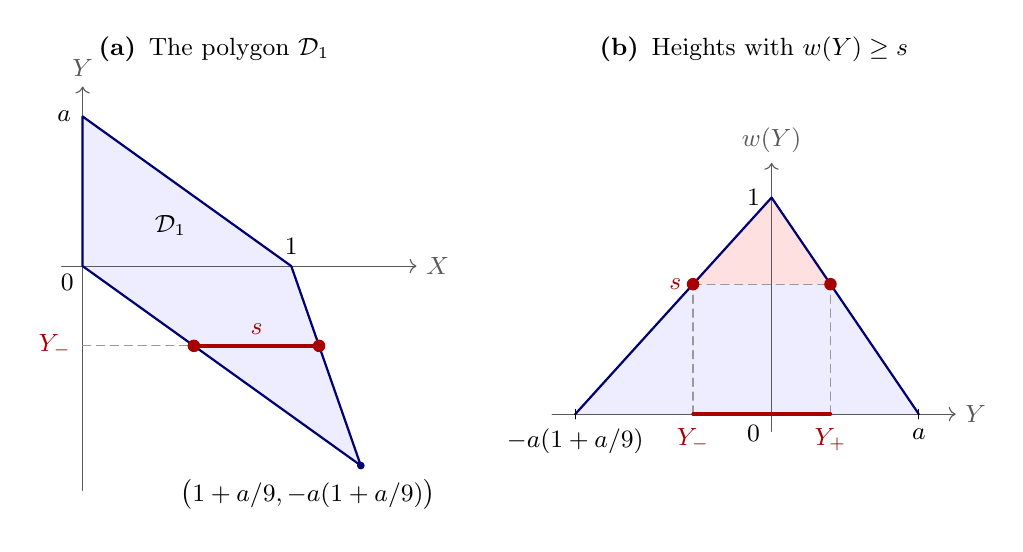
\begin{tikzpicture}[
  font=\small,
  line cap=round,
  line join=round,
  axis/.style={->,thin,black!65},
  boundary/.style={thick,blue!45!black},
  guide/.style={densely dashed,thin,black!40},
  sample/.style={very thick,red!65!black},
  slicepoint/.style={circle,inner sep=1.6pt,fill=red!65!black}
]
  \begin{scope}[x=2.65cm,y=1.90cm]
    \node[anchor=south] at (.63,1.30)
      {\textbf{(a)}\enspace The polygon $\mathcal D_1$};
    \fill[blue!7] (0,0)--(0,1)--(1,0)--(4/3,-4/3)--cycle;
    \draw[axis] (-.10,0)--(1.60,0) node[right] {$X$};
    \draw[axis] (0,-1.50)--(0,1.20) node[above] {$Y$};
    \draw[boundary] (0,0)--(0,1)--(1,0)--(4/3,-4/3)--cycle;
    \node[anchor=south west] at (.30,.14) {$\mathcal D_1$};
    \node[anchor=north east,inner sep=3pt] at (0,0) {$0$};
    \node[anchor=east,inner sep=4pt] at (0,1) {$a$};
    \node[anchor=south,inner sep=4pt] at (1,0) {$1$};
    \draw[guide] (0,-8/15)--(8/15,-8/15);
    \draw[sample] (8/15,-8/15)--(17/15,-8/15);
    \node[slicepoint] at (8/15,-8/15) {};
    \node[slicepoint] at (17/15,-8/15) {};
    \node[anchor=east,inner sep=4pt,text=red!65!black]
      at (0,-8/15) {$Y_-$};
    \node[anchor=south,inner sep=4pt,text=red!65!black]
      at (5/6,-8/15) {$s$};
    \fill[blue!45!black] (4/3,-4/3) circle (1.4pt);
    \node[anchor=north,inner sep=5pt] at (1.08,-4/3)
      {$\bigl(1+a/9,-a(1+a/9)\bigr)$};
  \end{scope}

  \begin{scope}[shift={(8.75cm,-1.88cm)},x=1.87cm,y=2.75cm]
    \node[anchor=south] at (-.12,1.58)
      {\textbf{(b)}\enspace Heights with $w(Y)\ge s$};
    \fill[blue!7] (-4/3,0)--(0,1)--(1,0)--cycle;
    \fill[red!12] (-8/15,3/5)--(0,1)--(2/5,3/5)--cycle;
    \draw[axis] (-1.49,0)--(1.25,0) node[right] {$Y$};
    \draw[axis] (0,-.08)--(0,1.16) node[above] {$w(Y)$};
    \draw[boundary] (-4/3,0)--(0,1)--(1,0);
    \draw[guide] (-8/15,0)--(-8/15,3/5);
    \draw[guide] (2/5,0)--(2/5,3/5);
    \draw[guide] (-8/15,3/5)--(2/5,3/5);
    \draw[sample] (-8/15,0)--(2/5,0);
    \node[slicepoint] at (-8/15,3/5) {};
    \node[slicepoint] at (2/5,3/5) {};
    \draw[thin] (-4/3,.022)--(-4/3,-.022);
    \draw[thin] (1,.022)--(1,-.022);
    \node[anchor=north,inner sep=5pt] at (-4/3,0)
      {$-a(1+a/9)$};
    \node[anchor=north,inner sep=5pt] at (1,0) {$a$};
    \node[anchor=north east,inner sep=4pt] at (0,0) {$0$};
    \node[anchor=east,inner sep=4pt] at (0,1) {$1$};
    \node[anchor=north,inner sep=5pt,text=red!65!black]
      at (-8/15,0) {$Y_-$};
    \node[anchor=north,inner sep=5pt,text=red!65!black]
      at (2/5,0) {$Y_+$};
    \node[anchor=east,inner sep=4pt,text=red!65!black]
      at (-8/15,3/5) {$s$};
  \end{scope}
\end{tikzpicture}

 \caption{Slice widths and their superlevel interval for
 $\mathcal D_1$, drawn schematically with $a=\rho_*$ and
 $0<s<1$. In panel~(a), the marked slice at
 $Y_-=-a(1+a/9)(1-s)$ has length $s$. In panel~(b), slices of
 length at least $s$ occur exactly at heights from $Y_-$ to
 $Y_+=a(1-s)$, an interval of length $q(1-s)$.
 Scaling by $m\lambda$ and translating by $(0,U_0)$ gives the
 polygon and height intervals used to bound the integer rows.}
 \label{fig:slice-profile}
\end{figure}

For each integer $K$, let
\[
 N_K=\#\{j\in\Z:(j,K)\in\mathcal S\}.
\]
Only finitely many of these row sizes are nonzero. The slice profile
in Figure~\ref{fig:slice-profile} bounds both each row size and the
number of rows of any given minimum size.
The passage from lengths to integer counts adds at most one endpoint.
We will absorb it with the size condition
\begin{equation}\label{eq:scaling}
 q(1-\lambda)m\ge1.
\end{equation}

\begin{lemma}[Integer row counts]\label{lem:integer-rows}
If $q(1-\lambda)m\ge1$, then the exponent set satisfies
\begin{equation}\label{eq:row-count}
 \begin{aligned}
 N_K&\le m &&(K\in\Z),\\
 \#\{K\in\Z:N_K\ge t\}
 &\le q(m-t+1) &&(1\le t\le m,\ t\in\Z).
 \end{aligned}
\end{equation}
\end{lemma}

\begin{proof}
By Lemmas~\ref{lem:exponent-enclosure} and~\ref{lem:slice-profile},
the integer positions in a represented row lie in an interval of
length at most $m\lambda<m$. Their span is at least $N_K-1$, so
integrality gives $N_K\le m$, also for a singleton row.

A row with $N_K\ge t$ requires a nonempty slice of length at least
$t-1$. If $t-1>m\lambda$, there are no such rows. Otherwise their
integer heights lie in a closed interval of length
$q(m\lambda-t+1)$. An interval of length $L\ge0$ contains at most
$\lfloor L\rfloor+1\le L+1$ integers. Therefore
\[
 \begin{aligned}
 \#\{K\in\Z:N_K\ge t\}
 &\le q(m\lambda-t+1)+1\\
 &=q(m-t+1)-q(1-\lambda)m+1\\
 &\le q(m-t+1)
 \end{aligned}
\]
by~\eqref{eq:scaling}. The extra one accounts for integral endpoints,
including when the height interval is a singleton.
\end{proof}

\subsection{Full rank and the strict inequality}

\begin{proposition}\label{prop:full-rank}
If $q(1-\lambda)m\ge1$, then the limiting matrix $B_0$
of~\eqref{eq:limiting-matrix} has full column rank. Consequently,
$J_\tau$ is injective for all sufficiently small positive $\tau$.
\end{proposition}

\begin{proof}
Apply Lemma~\ref{lem:interpolation} to $S=\mathcal S$, using
Lemma~\ref{lem:integer-rows}. The row vectors of $B_0$ are the
restrictions to $\mathcal S$ of the monomials spanning
$\mathcal P_{q,m}$. They therefore span $\C^{\mathcal S}$, so
$B_0$ has rank $\#\mathcal S$. Proposition~\ref{prop:matrix-limit}
then gives the injectivity of $J_\tau$ for sufficiently small $\tau$.
\end{proof}

\begin{proof}[Completion of the proof of Theorem~\ref{thm:main}]
By Lemma~\ref{lem:universal}, it suffices to exclude every universal
system $\mathsf U_r(d,m)$ with $d/m\le\sqrt r$.
Proposition~\ref{prop:squares} does so when $r$ is a square,
including equality.

For nonsquare $r$, the rational ratio $d/m$ is strictly below
$\sqrt r$, and Lemma~\ref{lem:cubic-low-degree} forces $d/m>3$.
Choose $\Delta$ as in~\eqref{eq:delta} and $\lambda$ as
in~\eqref{eq:lambda}. By Lemma~\ref{lem:universal}, replace
$(d,m)$ by a common positive integral multiple large enough to
satisfy~\eqref{eq:scaling}. The ratio $d/m$, and hence the choices
of $\rho$, $\Delta$, and $\lambda$, do not change. Apply all the
preceding constructions to this one chosen pair. Then
Proposition~\ref{prop:necessary-W} and Lemma~\ref{lem:collision}
give a nonzero kernel of $J_\tau$ for every fixed $\tau\in(0,1)$.
Proposition~\ref{prop:full-rank} gives an injective $J_\tau$ for
all sufficiently small positive $\tau$, a contradiction. The collision
has been taken on each fixed curve before the matrix limit; no
simultaneous choice of kernel vectors is needed.

There are therefore no universal systems of the required slope.
Lemma~\ref{lem:universal} supplies the single countable union $E_r$
and the strict inequality outside it, simultaneously for every
positive degree and every nonnegative integral multiplicity vector.
That reduction concerns all nonzero homogeneous forms, so the
conclusion includes reducible and nonreduced effective curves.
\end{proof}

\section{Fields and multipoint positivity}\label{sec:consequences}

The analytic proof was carried out over $\C$. Its conclusion extends by
algebraic incidence conditions, without embedding another field into
$\C$. The implication from complex Nagata to the corresponding statement
over uncountable algebraically closed characteristic-zero fields is also
discussed by Bansal--Majumder~\cite{BM2025}. We give the incidence
argument with the simultaneous quantifiers needed here.

\begin{corollary}\label{cor:fields}
Let $k$ be an uncountable algebraically closed field of characteristic
zero, and let $r\ge10$. There is a countable union of proper Zariski-closed
subsets of the space of distinct ordered $r$-tuples in $\Pp^2_k$, with
nonempty complement, outside which the conclusion of
Theorem~\ref{thm:main} holds with the same degree and multiplicity
conventions.
\end{corollary}
\begin{proof}
Let $A_{d,\mathbf m}$ be the $\mathbb Q$-defined incidence locus
constructed in the proof of Lemma~\ref{lem:universal}: its points are
the tuples admitting a nonzero degree-$d$ form with multiplicities at
least $\mathbf m$. On affine charts it is defined by the full-column-size
minors of the Taylor-coefficient matrix. The same rational minors define
its base change over any characteristic-zero field.

Whenever $d\sqrt r\le\sum_i m_i$, Theorem~\ref{thm:main} shows that
this locus is proper over $\C$. It is therefore proper over $\mathbb Q$
and remains proper over $k$: a nonzero defining minor on a rational affine
chart stays nonzero after field extension. Exclude these loci for all the
countably many violating pairs $(d,\mathbf m)$. Each tuple remaining
satisfies every asserted inequality. The complement is nonempty: choose
$2r$ affine coordinates in $k$ algebraically independent over $\mathbb Q$.
They avoid all these proper rationally defined loci and all coincidences.
Such coordinates exist by uncountability, since the algebraic closure in
$k$ of a field generated over $\mathbb Q$ by finitely many elements is
countable.
\end{proof}

Let $X$ be the blowup of the plane at a tuple covered by
Theorem~\ref{thm:main} or Corollary~\ref{cor:fields}. Write $H$ for the
pullback of a line and $E_1,\ldots,E_r$ for the exceptional curves.
A real divisor class is \emph{nef} if its intersection with every
irreducible curve is nonnegative, and \emph{strictly nef} if every such
intersection is positive. The multipoint Seshadri constant of the line
bundle $\mathcal O_{\Pp^2}(1)$ at the tuple is
\[
 \varepsilon(\mathcal O(1);p_1,\ldots,p_r)
 =\sup\{t\ge0:H-t\textstyle\sum_iE_i\text{ is nef}\}.
\]

\begin{corollary}\label{cor:sesha}
The class $N_r=\sqrt r\,H-\sum_iE_i$ is strictly nef and satisfies
$N_r^2=0$. In particular,
\[
 \varepsilon(\mathcal O(1);p_1,\ldots,p_r)=\frac1{\sqrt r}.
\]
\end{corollary}
\begin{proof}
Every irreducible curve on $X$ is either an exceptional curve or the
strict transform of an irreducible plane curve. The first kind has
intersection $1$ with $N_r$. For the second kind, the intersection is
$d\sqrt r-\sum_i\mult_{p_i}C>0$. Thus $N_r$ is strictly nef.
The intersection identities $H^2=1$, $H\cdot E_i=0$, and
$E_i\cdot E_j=-\delta_{ij}$ give $N_r^2=0$.

The class $H-r^{-1/2}\sum_iE_i$ is nef, so the Seshadri constant is
at least $r^{-1/2}$. For the opposite bound, fix a positive integer $n$ and put
$e_n=\lceil\sqrt r\,(n+1)\rceil$. There are at most
$r\binom{n+1}{2}$ linear conditions on degree-$e_n$ forms for
multiplicity at least $n$ at all the points, whereas
\[
 \binom{e_n+2}{2}>r\binom{n+1}{2}.
\]
Thus a nonzero such form exists. If $H-t\sum_iE_i$ is nef with
$t\ge0$, intersecting its class with the strict transform of this
form's divisor $D$ gives
\[
 0\le e_n-t\sum_i\mult_{p_i}D\le e_n-trn.
\]
Hence
$t\le e_n/(rn)$, which tends to $1/\sqrt r$ as $n\to\infty$.
This proves the upper bound using only the count of multiplicity
conditions.
\end{proof}

\bibliographystyle{plain}
\bibliography{references}
\end{document}
